\documentclass[a4paper, notitlepage]{article}
%\usepackage[cm]{fullpage}
\usepackage[pdftex]{graphicx}
\usepackage{wrapfig}
\usepackage{float}


\begin{document}

\title{Architecture} 
\date{\today}
\maketitle


This document briefly presents the internal organization of the system and identifies the high level components that it is built of. The organization of the system components is illustrated in Figure \ref{org}.
\bigskip

\begin{figure}[H]
  \centering
    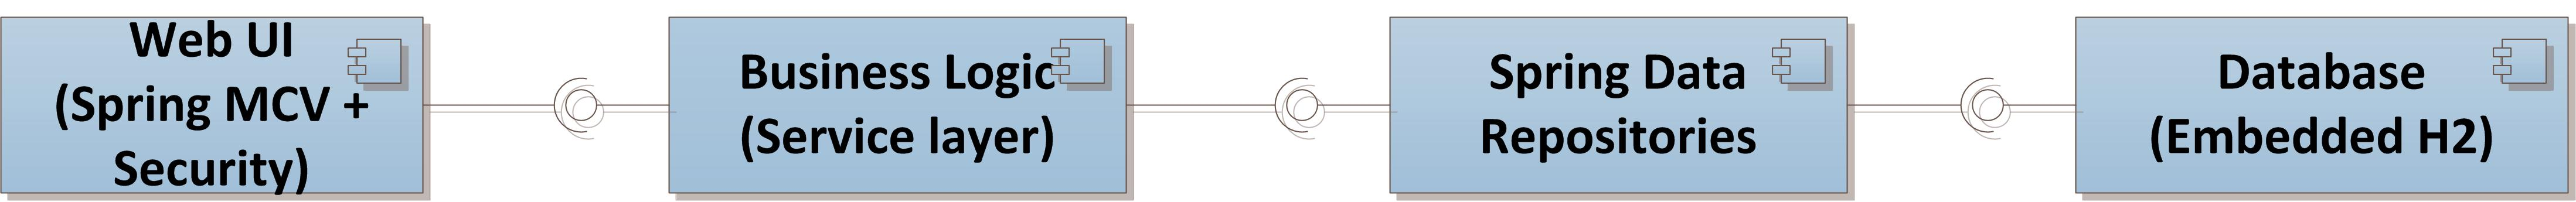
\includegraphics[width=1.3\textwidth]{high_level.jpg}
    \caption{Component diagram illustrating the functional organization of the system}
    \label{org}
\end{figure}


\bigskip
The architecture contains the following components:
\begin{itemize}
	\item \textit{Database} - Responsible to store the accounts and transactions data. In the current implementation we use embedded H2 database for simplicity but it is just a matter of configuration to switch to another SQL database. On startup the database is populated with some test data.
	
	\item \textit{Spring data repositories} - This component uses JPA2 and Hibernate to provide CRUD stile interaction with the database. The main application data objects (Person, Account, Transaction) are represented as JPA entities. 
	
	\item \textit{Business logic} - This component defines the Spring services which encapsulate the main business logic of the application.
	
	\item \textit{Web UI} - This component is responsible to provide the Web interface of the application. It uses Spring MVC in combination with Thymeleaf and Apache Tiles to render the views presented to the users. The application also uses Spring Security to manage the access to its functionality. It uses the user information from the database (Person) for authentication.
\end{itemize}

\end{document}